%!TEX TS-program = xelatex
%!TEX encoding = UTF-8 Unicode

%%%  Syllabus template for use with style files at http://kjhealy.github.com/latex-custom-kjh
%%%  Kieran Healy

\documentclass[11pt,article,oneside]{memoir}

% packages
\usepackage{org-preamble-xelatex}
\usepackage{wallpaper}
\usepackage{xcolor}
\usepackage{enumitem}
\usepackage{multicol}
\setlength{\columnsep}{1em}
\usepackage{booktabs}
\newcommand{\ra}[1]{\renewcommand{\arraystretch}{#1}}

\AtBeginBibliography{\small}

% Definitions
\def\myauthor{Author}
\def\mytitle{Title}
\def\mycopyright{\myauthor}
\def\mykeywords{}
\def\mybibliostyle{plain}
\def\mybibliocommand{}
\def\mysubtitle{}
\def\myaffiliation{Louisiana State University}
\def\myaddress{309 Design}
\def\myemail{baharmon@lsu.edu} 
\def\myweb{https://baharmon.github.io/}
\def\myphone{919.622.8414}
\def\myversion{}
\def\myrevision{}
\def\myaffiliation{\ \\Louisiana State University}
\def\myauthor{Brendan Harmon}
\def\mykeywords{Landscape Architecture, Syllabus}
\def\mytitle{{\normalsize \textsc{LA} 2101 | 7102\newline} \huge \bfseries Landscape Representation}
% Landscape Representation III \& Graduate Landscape Representation II
\def\mysubtitle{\Large FRANK LLOYD WRIGHT'S Unbuilt Houses}

% color
\makeatletter
\newcommand{\globalcolor}[1]{%
  \color{#1}\global\let\default@color\current@color
}
\makeatother

% begin
\begin{document}

\setlength\bibitemsep{0.75em}

% fonts
\defaultfontfeatures{}
\defaultfontfeatures{Scale=MatchLowercase}         
\setmainfont[Scale=1, Path = fonts/lato/,BoldItalicFont=Lato-RegIta,BoldFont=Lato-Reg,ItalicFont=Lato-LigIta]{Lato-Lig}
%\setmainfont[Scale=1, Path = fonts/eaglefeather/,BoldItalicFont=Eaglefeather-Bold Italic,BoldFont=Eaglefeather-Bold,ItalicFont=Eaglefeather-Italic]{Eaglefeather}
%\setsansfont[Scale=1, Path = fonts/lato/,BoldItalicFont=Lato-RegIta,BoldFont=Lato-Reg,ItalicFont=Lato-LigIta]{Lato-Lig}
\setsansfont[Scale=1, Path = fonts/eaglefeather/,BoldItalicFont=Eaglefeather-Bold Italic,BoldFont=Eaglefeather-Bold,ItalicFont=Eaglefeather-Italic]{Eaglefeather}
\setmonofont[Mapping=tex-text,Scale=0.8,Path = fonts/inconsolata/]{i}

\def\ind{\hangindent=1 true cm\hangafter=1 \noindent}
\def\labelitemi{$\cdot$}
\chapterstyle{article-4-sans}  
\title{\LARGE \mytitle \newline \mysubtitle}     
\author{\Large\myauthor \newline \footnotesize\texttt{\noindent\myemail}}
\date{Spring 2018. Design 217.\newline Monday, Wednesday, \& Friday 9:30am--11:30am.}
\published{\,}

% -------------------------------- COVER PAGE -------------------------------- 

\pagenumbering{gobble}
\globalcolor{black}
\vspace*{-10em}
\maketitle
\ThisCenterWallPaper{1}{../images/morris_cover.jpg}
\vfill
\begin{center}
\noindent \textbf{Morris House} \\
%\copyright \hspace*{0.25em} 
Frank Lloyd Wright \\
\footnotesize{1945}
\end{center}
\clearpage

% -------------------------------- DESCRIPTION -------------------------------- 

\pagenumbering{arabic}
\globalcolor{black}
\vspace*{-10em}
\maketitle

\section{Course Description}
%\section{COURSE DESCRIPTION}
%
This course is an introduction to 3D modeling for landscape architects. 
%%
In this course you will develop a solid foundation in 3D modeling
by building a detailed digital model of one of 
Frank Lloyd Wright's unbuilt houses and its landscape. 
%
You will learn a range of 3D modeling techniques including
3D drafting, solid modeling, surface modeling,  mesh modeling, and billboards. 
%
You will learn how to digital fabricate physical models 
of buildings and landscapes using 3D printing. 
%
You will also learn how to make graphics with
3D rendering and photomontage.
%
Each week you will spend a day in a workshop
learning new methods
and a day developing your projects.
%
You will work in small teams and 
will present an exhibition and a booklet of your
models and renderings at the end of the course.\\

\section{Optional Fieldtrip}
There will be an optional fieldtrip to New York City 
to view the Frank Lloyd Wright Collection 
at Columbia's Avery Architectural and Fine Arts Library 
led by Prof.~Desmond. 

\clearpage

% -------------------------------- FIGURES -------------------------------- 

\begin{figure}
\begin{center}
%
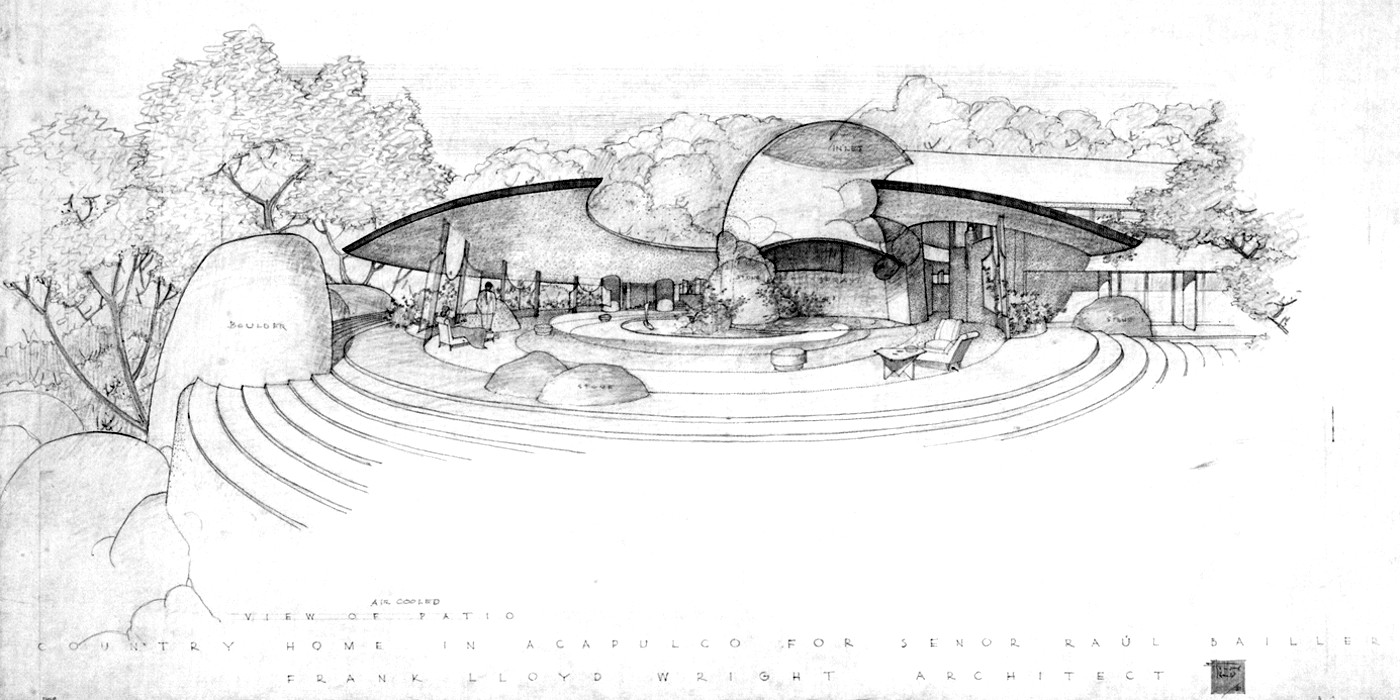
\includegraphics[width=0.9\textwidth]{../images/bailleres_1_greyscale.jpg}
\caption{Bailleres House, Acapulco, Mexico, 1952}
%
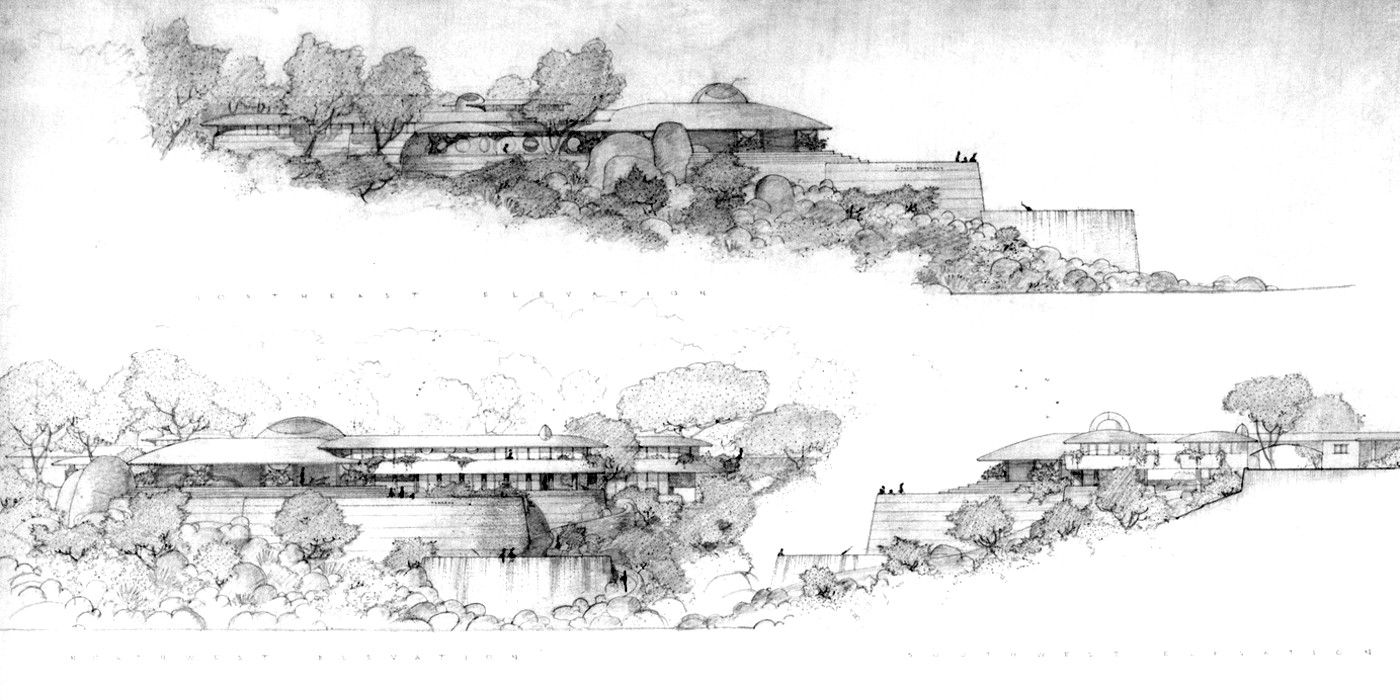
\includegraphics[width=0.9\textwidth]{../images/bailleres_2_greyscale.jpg}
\caption{Bailleres House, Acapulco, Mexico, 1952}
%
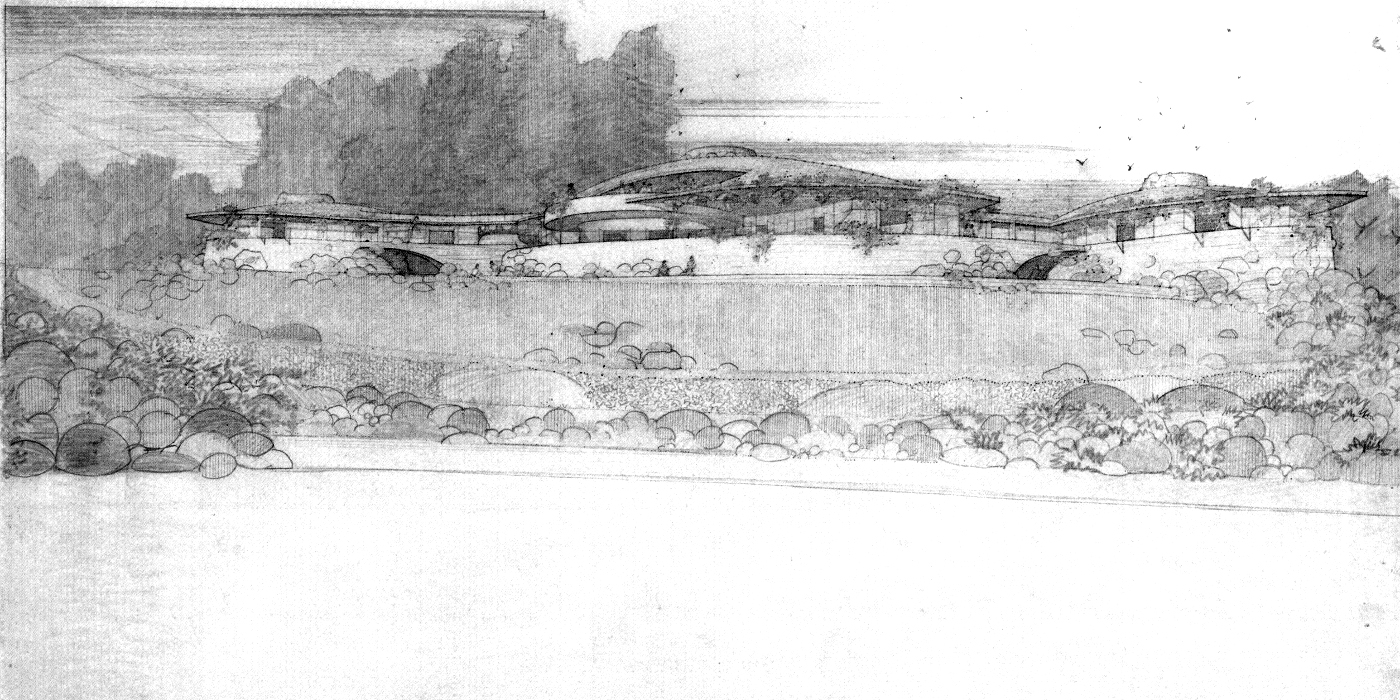
\includegraphics[width=0.9\textwidth]{../images/boulder_greyscale.jpg}
\caption{Kaufman Boulder House, Palm Springs, CA, USA, 1950}
%
%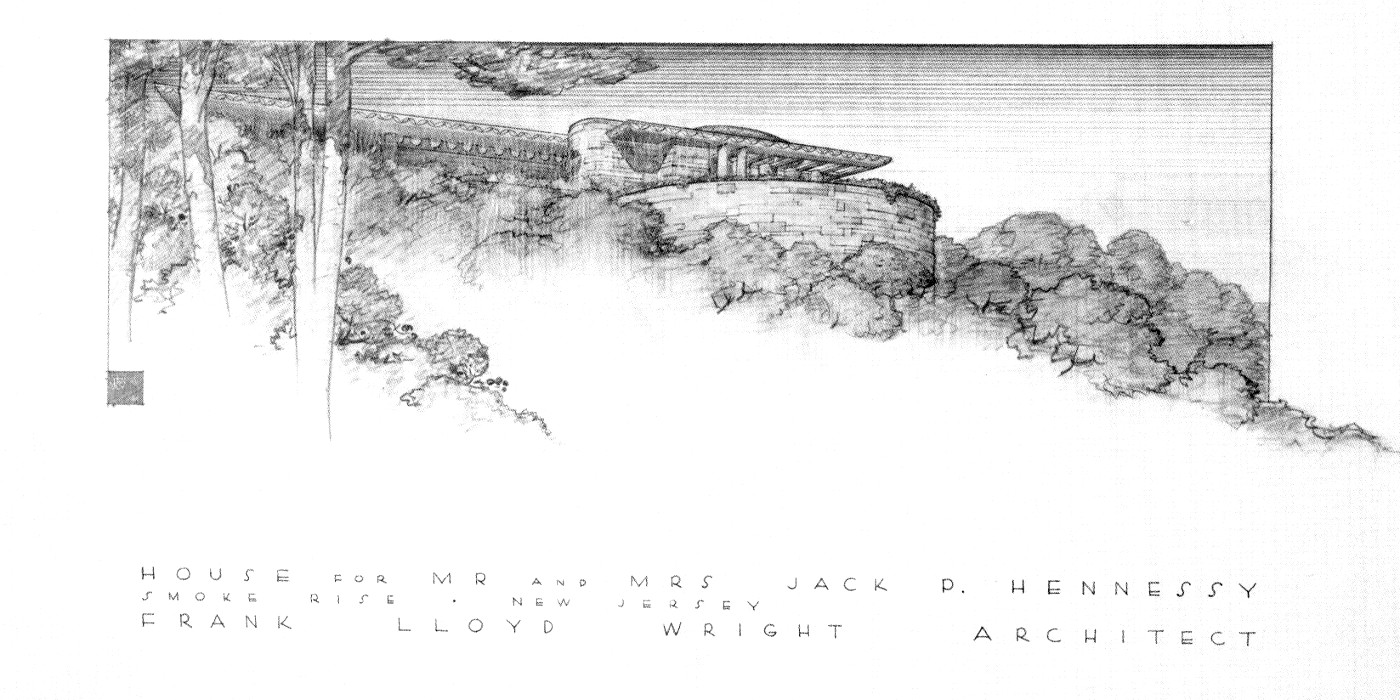
\includegraphics[width=\textwidth]{../images/hennesey_greyscale.jpg}
%\caption{Hennesey House, 1956}
%
%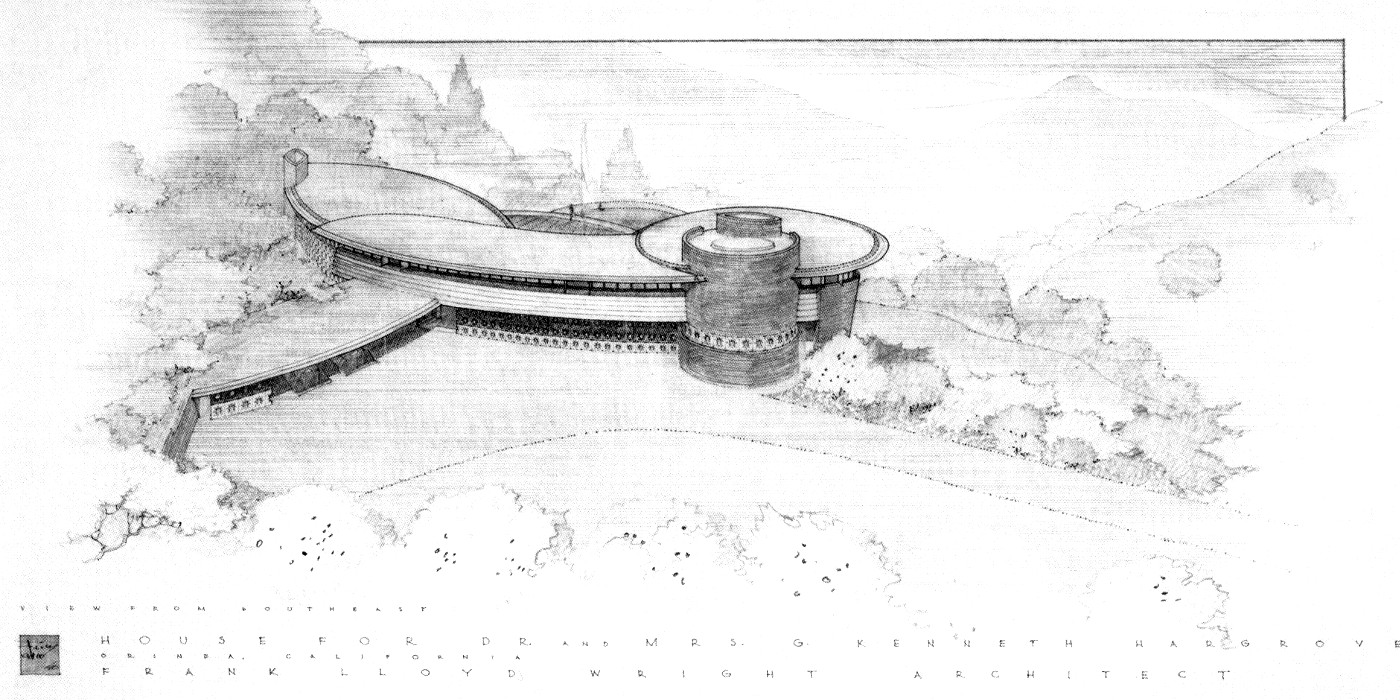
\includegraphics[width=\textwidth]{../images/hargrove_1_greyscale.jpg}
%%\caption{Hargrove House, 1950}
%
\label{fig:unbuilt_houses}
\end{center}
\end{figure}

\clearpage

% -------------------------------- SCHEDULE -------------------------------- 

\section{Course Schedule}
%\section{COURSE SCHEDULE}

\begin{multicols}{3}
\begin{enumerate}[label=\textbf{\arabic*}]
%
\item Seminar
\item 2D-3D drafting
\item Solid modeling
\item Surface modeling
\item Data acquisition
\item Terrain modeling
\item 3D rendering
\item Section-elevations
\item 3D printing
\item Billboard trees
\item Photomontage
\item Layout design
\item Production
%
\item Booklet
\item Exhibition
%
\end{enumerate}
\end{multicols}

%\clearpage

% -------------------------------- PROJECTS -------------------------------- 
\section{Projects}
As groups % of x
you will 3D model of one of 
Frank Lloyd Wright's unbuilt houses or estates
-- either Jester House, Usonia, Morris House, Galesburg, 
Hargrove House, Kaufman Boulder House, Bailleres House, 
Hennesey House, or Stillman House -- 
and its landscape.\\

\noindent \textbf{3D Renderings}
Each group will create beautiful 3D renderings
of their house and its landscape. 
These renderings should include 
a plan,
a sun study, 
4 section-elevations, 
and 4 perspectives.\\

\noindent \textbf{3D Prints}
Each group will make a beautiful 3D printed model 
of their building and its topography.
The model should be printed in multiple parts
to reveal sectional views.\\

\noindent \textbf{Booklet}
Each group will prepare a booklet for the exhibition 
about the house, the site, the clients, the original drawings, 
your 3D renderings, and photos of your 3D prints.\\

\noindent \textbf{Exhibition}
Each group will create a display for 
an exhibition of the unbuilt houses.
Each display should include
plots of your 3D renderings,
your 3D prints, and 
information about the house.\\

\clearpage

% -------------------------------- Software -------------------------------- 
\section{Software}
Rhinoceros | \url{https://www.rhino3d.com/}\\
RhinoTerrain | \url{http://www.rhinoterrain.com/}\\
ArcGIS | \url{http://desktop.arcgis.com/en/}\\
Adobe Photoshop | \url{http://www.adobe.com/products/photoshop.html}\\
Adobe Illustrator | \url{http://www.adobe.com/products/illustrator.html}\\
Adobe InDesign | \url{http://www.adobe.com/products/indesign.html}\\
Blender | \url{https://www.blender.org/}\\

% -------------------------------- Grading -------------------------------- 
\section{Grading}

\begin{table}[H]
\small
\begin{tabular}{l l l l l l l l}
\textbf{3D Renderings} & 25\% &
\textbf{3D Prints} & 25\% &
\textbf{Exhibition} & 25\% &
\textbf{Booklet} & 25\% \\
\end{tabular}
\end{table}

% -------------------------------- Readings -------------------------------- 
\section{Readings}
\renewcommand*{\bibfont}{\normalsize} %\small
\vspace*{0.5cm}
\nocite{*}
\setlength\bibitemsep{1\baselineskip}
\printbibliography[heading=none]

%\clearpage

% -------------------------------- Policies -------------------------------- 
\section{Policies}

\noindent \textbf{Communication Intensive}
This is a certified Communication-Intensive (C-I) course,
which meets all of the requirements set
forth by LSU’s Communication across the Curriculum program, including
 instruction and assignments emphasizing
informal and formal visual and technological communication,
teaching of discipline-specific communication techniques,
use of feedback loops for learning,
40\% of the course grade rooted in communication-based work, and
practice of ethical and professional work standards.
Students interested in pursuing the LSU Distinguished Communicators 
certification may use this C-I course for credit. 
For more information about this student recognition program visit: 
\url{www.cxc.lsu.edu}.\\

\clearpage

\noindent \textbf{Time Commitment Expectations}
LSU's general policy states that for each credit hour, you (the student) should plan to
spend at least two hours working on course related activities outside of class. Since this course is for three credit hours, you should expect to spend a minimum of six hours outside of class each week working on assignments for this course. For more information see: 
\url{http://catalog.lsu.edu/content.php?catoid=12&navoid=822}.\\

\noindent \textbf{LSU student code of conduct}
The LSU student code of conduct explains student rights, excused absences, and what is expected of student behavior. Students are expected to understand this code:  \url{http://students.lsu.edu/saa/students/code}.\\ %Any violations of the LSU student code will be duly reported to the Dean of Students.\\

\noindent \textbf{Disability Code}
The University is committed to making reasonable efforts to assist individuals with disabilities in
their efforts to avail themselves of services and programs offered by the University. To this end,
Louisiana State University will provide reasonable accommodations for persons with
documented qualifying disabilities. If you have a disability and feel you need accommodations in
this course, you must present a letter to me from Disability Services in 115 Johnston Hall,
indicating the existence of a disability and the suggested accommodations.\\

\noindent \textbf{Academic Integrity}
According to section 10.1 of the LSU Code of Student Conduct, ``A student may be charged with Academic Misconduct'' for a variety of offenses, including the following: unauthorized copying, collusion, or collaboration; ``falsifying'' data or citations; ``assisting someone in the commission or attempted commission of an offense''; and plagiarism, which is defined in section 10.1.H as a ``lack of appropriate citation, or the unacknowledged inclusion of someone else's words, structure, ideas, or data; failure to identify a source, or the submission of essentially the same work for two assignments without permission of the instructor(s).''\\

\noindent \textbf{Plagiarism and Citation Method}
Plagiarism is the ``lack of appropriate citation, or the unacknowledged inclusion of someone else's words, structure, ideas, or data; failure to identify a source, or the submission of essentially the same work for two assignments without permission of the instructor(s)'' (Sec. 10.1.H of the LSU Code of Student Conduct). As a student at LSU, it is your responsibility to refrain from plagiarizing the academic property of another and to utilize appropriate citation method for all coursework. In this class, it is recommended that you use Chicago Style author-date citations. Ignorance of the citation method is not an excuse for academic misconduct.


\end{document}
